\documentclass[twoside]{book}

% Packages required by doxygen
\usepackage{calc}
\usepackage{doxygen}
\usepackage{graphicx}
\usepackage[utf8]{inputenc}
\usepackage{makeidx}
\usepackage{multicol}
\usepackage{multirow}
\usepackage{textcomp}
\usepackage[table]{xcolor}

% Font selection
\usepackage[T1]{fontenc}
\usepackage{mathptmx}
\usepackage[scaled=.90]{helvet}
\usepackage{courier}
\usepackage{amssymb}
\usepackage{sectsty}
\renewcommand{\familydefault}{\sfdefault}
\allsectionsfont{%
  \fontseries{bc}\selectfont%
  \color{darkgray}%
}
\renewcommand{\DoxyLabelFont}{%
  \fontseries{bc}\selectfont%
  \color{darkgray}%
}

% Page & text layout
\usepackage{geometry}
\geometry{%
  a4paper,%
  top=2.5cm,%
  bottom=2.5cm,%
  left=2.5cm,%
  right=2.5cm%
}
\tolerance=750
\hfuzz=15pt
\hbadness=750
\setlength{\emergencystretch}{15pt}
\setlength{\parindent}{0cm}
\setlength{\parskip}{0.2cm}
\makeatletter
\renewcommand{\paragraph}{%
  \@startsection{paragraph}{4}{0ex}{-1.0ex}{1.0ex}{%
    \normalfont\normalsize\bfseries\SS@parafont%
  }%
}
\renewcommand{\subparagraph}{%
  \@startsection{subparagraph}{5}{0ex}{-1.0ex}{1.0ex}{%
    \normalfont\normalsize\bfseries\SS@subparafont%
  }%
}
\makeatother

% Headers & footers
\usepackage{fancyhdr}
\pagestyle{fancyplain}
\fancyhead[LE]{\fancyplain{}{\bfseries\thepage}}
\fancyhead[CE]{\fancyplain{}{}}
\fancyhead[RE]{\fancyplain{}{\bfseries\leftmark}}
\fancyhead[LO]{\fancyplain{}{\bfseries\rightmark}}
\fancyhead[CO]{\fancyplain{}{}}
\fancyhead[RO]{\fancyplain{}{\bfseries\thepage}}
\fancyfoot[LE]{\fancyplain{}{}}
\fancyfoot[CE]{\fancyplain{}{}}
\fancyfoot[RE]{\fancyplain{}{\bfseries\scriptsize Generated on Wed Jun 4 2014 20\-:21\-:48 for Projekt\-\_\-znajomi by Doxygen }}
\fancyfoot[LO]{\fancyplain{}{\bfseries\scriptsize Generated on Wed Jun 4 2014 20\-:21\-:48 for Projekt\-\_\-znajomi by Doxygen }}
\fancyfoot[CO]{\fancyplain{}{}}
\fancyfoot[RO]{\fancyplain{}{}}
\renewcommand{\footrulewidth}{0.4pt}
\renewcommand{\chaptermark}[1]{%
  \markboth{#1}{}%
}
\renewcommand{\sectionmark}[1]{%
  \markright{\thesection\ #1}%
}

% Indices & bibliography
\usepackage{natbib}
\usepackage[titles]{tocloft}
\setcounter{tocdepth}{3}
\setcounter{secnumdepth}{5}
\makeindex

% Hyperlinks (required, but should be loaded last)
\usepackage{ifpdf}
\ifpdf
  \usepackage[pdftex,pagebackref=true]{hyperref}
\else
  \usepackage[ps2pdf,pagebackref=true]{hyperref}
\fi
\hypersetup{%
  colorlinks=true,%
  linkcolor=blue,%
  citecolor=blue,%
  unicode%
}

% Custom commands
\newcommand{\clearemptydoublepage}{%
  \newpage{\pagestyle{empty}\cleardoublepage}%
}


%===== C O N T E N T S =====

\begin{document}

% Titlepage & ToC
\hypersetup{pageanchor=false}
\pagenumbering{roman}
\begin{titlepage}
\vspace*{7cm}
\begin{center}%
{\Large Projekt\-\_\-znajomi \\[1ex]\large 1.\-01 }\\
\vspace*{1cm}
{\large Generated by Doxygen 1.8.6}\\
\vspace*{0.5cm}
{\small Wed Jun 4 2014 20:21:48}\\
\end{center}
\end{titlepage}
\clearemptydoublepage
\tableofcontents
\clearemptydoublepage
\pagenumbering{arabic}
\hypersetup{pageanchor=true}

%--- Begin generated contents ---
\chapter{Wyszukiwanie znajomości}
\label{index}\hypertarget{index}{}\begin{DoxyAuthor}{Author}
Pawel Zurek 
\end{DoxyAuthor}
\begin{DoxyDate}{Date}
16.\-03.\-2014 
\end{DoxyDate}
\begin{DoxyVersion}{Version}
1.\-1.\-b
\end{DoxyVersion}
Program umożliwia liczenie czasu trwania operacji wypelniania liczbami stosu / kolejki.\hypertarget{index_etykieta-wazne-cechy}{}\section{Najważniejsze cechy}\label{index_etykieta-wazne-cechy}
Program sluzy do liczenia czasu wypelnienia liczbami stosow i kolejek za pomoca \-:\par


\par
-\/$>$ list \par
-\/$>$ tablic ( po przekroczeniu rozmiaru tablicy, rozmiar powiekszany o jeden ) \par
-\/$>$ tablic ( po przekroczeniu rozmiaru tablicy, rozmiar zwiekszany dwukrotnie )\hypertarget{index_etykieta-op-algorytm}{}\section{Opis algorytmu}\label{index_etykieta-op-algorytm}
Algorytm w tym zadaniu to 6 petli \-: \par
-\/$>$ wypelnienie stosu za pomoca listy \par
-\/$>$ wypelnienie kolejki za pomoca listy \par
-\/$>$ wypelnienie stosu za pomoca tablicy ( rozmiar o jeden ) \par
-\/$>$ wypelnienie stosu za pomoca tablicy ( rozmiar x2 ) \par
-\/$>$ wypelnienie kolejki za pomoca tablicy ( rozmiar o jeden ) \par
-\/$>$ wypelnienie kolejki za pomoca tablicy ( rozmiar x2)

\par
,na ktora sklada sie wypelnienie nastepujaca iloscia elementow\-:

\par
-\/$>$ 10 \par
-\/$>$ 100 \par
-\/$>$ 1000 \par
-\/$>$ 10000

Czasy sa wyprowadzane na standartowe wyjscie. 
\chapter{Class Index}
\section{Class List}
Here are the classes, structs, unions and interfaces with brief descriptions\-:\begin{DoxyCompactList}
\item\contentsline{section}{\hyperlink{class_graf}{Graf} \\*Modeluje pojecie graf. Klasa sluzy glownie do wykonania algorytmu wyszukiwania, czyli znalezienia polaczenia miedzy dwoma punktami }{\pageref{class_graf}}{}
\item\contentsline{section}{\hyperlink{structpor}{por} \\*Struktura porownywania Struktura ta ma na celu ulatwienie dzialania algorytmu wyszukiwania ( Dijkstry ) Prownuje ona wartosci drogi miedzy dwoma wezlami }{\pageref{structpor}}{}
\item\contentsline{section}{\hyperlink{struct_wezel}{Wezel} \\*Struktura Wezla Struktura ta ma zdefiniowane dwie zmienne nr oraz g, ktore odpowiadaja za przechowywanie numer wierzcholkana oraz droge jaka juz przebyl od poczatku dzialania wyszukiwania }{\pageref{struct_wezel}}{}
\item\contentsline{section}{\hyperlink{class_wierzcholek}{Wierzcholek} \\*Definicje dla klasy \hyperlink{class_wierzcholek}{Wierzcholek} Struktura ta ma zdefiniowane dwie zmienne sasiad oraz waga. Przy wczytywaniu pliku dodajac wierzcholek dodajemy odrazu informacje o aktualnym sasiedzie oraz o wadze polaczenia miedzy wierzcholkiem i sasiadem }{\pageref{class_wierzcholek}}{}
\end{DoxyCompactList}

\chapter{File Index}
\section{File List}
Here is a list of all files with brief descriptions\-:\begin{DoxyCompactList}
\item\contentsline{section}{/home/pawel/\-Dokumenty/programowanie/pamsi/projekt\-\_\-znajomi/prj/inc/\hyperlink{_dijkstry_8hh}{Dijkstry.\-hh} \\*Definicje funkcji dla klasy graf }{\pageref{_dijkstry_8hh}}{}
\item\contentsline{section}{/home/pawel/\-Dokumenty/programowanie/pamsi/projekt\-\_\-znajomi/prj/src/\hyperlink{_dijkstry_8cpp}{Dijkstry.\-cpp} \\*Plik zawiera funkcje z klasy graf }{\pageref{_dijkstry_8cpp}}{}
\item\contentsline{section}{/home/pawel/\-Dokumenty/programowanie/pamsi/projekt\-\_\-znajomi/prj/src/\hyperlink{main_8cpp}{main.\-cpp} \\*Plik zawiera funkcje \hyperlink{main_8cpp_ae66f6b31b5ad750f1fe042a706a4e3d4}{main()} }{\pageref{main_8cpp}}{}
\end{DoxyCompactList}

\chapter{Class Documentation}
\hypertarget{class_graf}{\section{Graf Class Reference}
\label{class_graf}\index{Graf@{Graf}}
}


Modeluje pojecie graf. Klasa sluzy glownie do wykonania algorytmu wyszukiwania, czyli znalezienia polaczenia miedzy dwoma punktami.  




{\ttfamily \#include $<$Dijkstry.\-hh$>$}

\subsection*{Public Member Functions}
\begin{DoxyCompactItemize}
\item 
\hyperlink{class_graf_a05a504069321858769df57555045d808}{Graf} ()
\begin{DoxyCompactList}\small\item\em Konstruktor klasy \hyperlink{class_graf}{Graf}. \end{DoxyCompactList}\item 
\hyperlink{class_graf_a4ff3904fd04f367ac0219b52719c567e}{$\sim$\-Graf} ()
\begin{DoxyCompactList}\small\item\em Destruktor klasy \hyperlink{class_graf}{Graf}. \end{DoxyCompactList}\item 
void \hyperlink{class_graf_a2fe84bc61e57b1712687af6bda740103}{generuj\-\_\-liste} (int ilosc, int gestosc)
\begin{DoxyCompactList}\small\item\em Funkcja generujaca \hyperlink{class_graf}{Graf}. \end{DoxyCompactList}\item 
void \hyperlink{class_graf_adaba0ec276dc425b2556f2dadae7845f}{stworz\-\_\-liste\-\_\-z\-\_\-pliku} (string nazwapliku)
\begin{DoxyCompactList}\small\item\em Funkcja tworzaca \hyperlink{class_graf}{Graf} z pliku. \end{DoxyCompactList}\item 
void \hyperlink{class_graf_a3fee2a8a88543338f1d54216c2618e2b}{stworz\-\_\-wierzcholki} (string nazwapliku)
\begin{DoxyCompactList}\small\item\em Funkcja tworzaca wierzcholki \hyperlink{class_graf}{Graf} u z pliku. \end{DoxyCompactList}\item 
void \hyperlink{class_graf_a7997ef54e93c3b83a2435bfd0d4c51c8}{przerob\-\_\-z\-\_\-fb} (string typ, string wyjscie)
\begin{DoxyCompactList}\small\item\em Funkcja przerabiajaca plik z bazy . \end{DoxyCompactList}\item 
void \hyperlink{class_graf_ab1baac77bf17276ab97c721536dc4f33}{dowolny\-\_\-plik} ()
\begin{DoxyCompactList}\small\item\em Funkcja pomocnicza do main . \end{DoxyCompactList}\item 
void \hyperlink{class_graf_a550437f8c2066ea035644502c93e1b7d}{domyslny\-\_\-plik} ()
\begin{DoxyCompactList}\small\item\em Funkcja pomocnicza do main . \end{DoxyCompactList}\item 
void \hyperlink{class_graf_a8a0677ac53fdef2117a52da0f944701a}{testowy\-\_\-plik} ()
\begin{DoxyCompactList}\small\item\em Funkcja pomocnicza do main . \end{DoxyCompactList}\item 
void \hyperlink{class_graf_aa66538b00c1915825b1e83339294c44e}{losowe\-\_\-dijkstry} ()
\begin{DoxyCompactList}\small\item\em Funkcja pomocnicza do main . \end{DoxyCompactList}\item 
bool \hyperlink{class_graf_ad83cd4b8656ccb75bd7b5f6cfe779080}{czy\-\_\-spojny} ()
\begin{DoxyCompactList}\small\item\em Funkcja pomocnicza. \end{DoxyCompactList}\item 
bool \hyperlink{class_graf_a2cefd6ebc3329cd029351d1509eadd7a}{czy\-\_\-poprawne} (int a, int b)
\begin{DoxyCompactList}\small\item\em Funkcja pomocnicza. \end{DoxyCompactList}\item 
bool \hyperlink{class_graf_a799ce938ca34db184e4ac0598f58398f}{czy\-\_\-bylo} (int v1, int v2)
\begin{DoxyCompactList}\small\item\em Funkcja pomocnicza. \end{DoxyCompactList}\item 
int \hyperlink{class_graf_ae3cb2f3d4a8c9cc67845eacacf6a612d}{przypisz\-\_\-indeks} (int id)
\begin{DoxyCompactList}\small\item\em Funkcja pomocnicza. \end{DoxyCompactList}\item 
int \hyperlink{class_graf_ad85c82918ac15887c9e423cd4edb1dba}{dijkstry} (int a, int b)
\begin{DoxyCompactList}\small\item\em Funkcja glowna programu wyszukujaca polaczenie. \end{DoxyCompactList}\item 
void \hyperlink{class_graf_a3a084b33cfcfa17bbfc05570043aaab2}{wyswietl} ()
\begin{DoxyCompactList}\small\item\em Funkcja wyswietlajaca liste sasiedztwa grafu. \end{DoxyCompactList}\end{DoxyCompactItemize}
\subsection*{Public Attributes}
\begin{DoxyCompactItemize}
\item 
int \hyperlink{class_graf_a673185b62d4c232bcbbc0200e95e7481}{V}
\begin{DoxyCompactList}\small\item\em Pole typu int, bedzie uzywane do przechowywania informacji o ilosci wierzcholkow. \end{DoxyCompactList}\item 
int \hyperlink{class_graf_a30dc3bf4726fbd2d056c98f15080b236}{E}
\begin{DoxyCompactList}\small\item\em Pole typu int, bedzie uzywane do przechowywania informacji o ilosci krawedzi (aktualnie nie uzywane w programie ). \end{DoxyCompactList}\item 
vector$<$ \hyperlink{class_wierzcholek}{Wierzcholek} $>$ $\ast$ \hyperlink{class_graf_adf576dd4fd3cb35f4328a66befaa9c7a}{lista\-\_\-sasiadujaca}
\begin{DoxyCompactList}\small\item\em Pole typu $\ast$ vector, bedzie uzywane do przechowywania informacji o sasiadach dla poszczegolnych wierzcholkow. \end{DoxyCompactList}\item 
int $\ast$ \hyperlink{class_graf_a2df9c551c0ed169e20bdfe06aba56558}{wierzcholki}
\begin{DoxyCompactList}\small\item\em Pole typu $\ast$ int, bedzie uzywane jako wektor z prawdziwymi nazwami (id) wierzcholkow. \end{DoxyCompactList}\end{DoxyCompactItemize}


\subsection{Detailed Description}
Modeluje pojecie graf. Klasa sluzy glownie do wykonania algorytmu wyszukiwania, czyli znalezienia polaczenia miedzy dwoma punktami. 

Definition at line 76 of file Dijkstry.\-hh.



\subsection{Constructor \& Destructor Documentation}
\hypertarget{class_graf_a05a504069321858769df57555045d808}{\index{Graf@{Graf}!Graf@{Graf}}
\index{Graf@{Graf}!Graf@{Graf}}
\subsubsection[{Graf}]{\setlength{\rightskip}{0pt plus 5cm}Graf\-::\-Graf (
\begin{DoxyParamCaption}
{}
\end{DoxyParamCaption}
)}}\label{class_graf_a05a504069321858769df57555045d808}


Konstruktor klasy \hyperlink{class_graf}{Graf}. 

Konstruktor jest bezparametryczny. Jedyne jego zadanie to zainicjalizowanie zmiennych wewnetrznych klasy \hyperlink{class_graf}{Graf} 

Definition at line 12 of file Dijkstry.\-cpp.

\hypertarget{class_graf_a4ff3904fd04f367ac0219b52719c567e}{\index{Graf@{Graf}!$\sim$\-Graf@{$\sim$\-Graf}}
\index{$\sim$\-Graf@{$\sim$\-Graf}!Graf@{Graf}}
\subsubsection[{$\sim$\-Graf}]{\setlength{\rightskip}{0pt plus 5cm}Graf\-::$\sim$\-Graf (
\begin{DoxyParamCaption}
{}
\end{DoxyParamCaption}
)}}\label{class_graf_a4ff3904fd04f367ac0219b52719c567e}


Destruktor klasy \hyperlink{class_graf}{Graf}. 

Destruktor jest bezparametryczny. Jedyne jego zadanie to usuniecie obiektow zaalokowanych dynamicznie 

Definition at line 15 of file Dijkstry.\-cpp.



\subsection{Member Function Documentation}
\hypertarget{class_graf_a799ce938ca34db184e4ac0598f58398f}{\index{Graf@{Graf}!czy\-\_\-bylo@{czy\-\_\-bylo}}
\index{czy\-\_\-bylo@{czy\-\_\-bylo}!Graf@{Graf}}
\subsubsection[{czy\-\_\-bylo}]{\setlength{\rightskip}{0pt plus 5cm}bool Graf\-::czy\-\_\-bylo (
\begin{DoxyParamCaption}
\item[{int}]{v1, }
\item[{int}]{v2}
\end{DoxyParamCaption}
)}}\label{class_graf_a799ce938ca34db184e4ac0598f58398f}


Funkcja pomocnicza. 

Funkcja sprawdza czy dane wierzcholki juz sa w bazie aby nie wpisywac ich ponownie 
\begin{DoxyParams}{Parameters}
{\em v1} & -\/$>$ pole typu int z id drugiego wierzcholka \\
\hline
{\em v2} & -\/$>$ pole typu int z id pierwszego wierzcholka \\
\hline
\end{DoxyParams}
\begin{DoxyReturn}{Returns}
1 -\/$>$ gdy wierzcholki sa w bazie 0 -\/$>$ gdy wierzcholkow nie ma w bazie 
\end{DoxyReturn}


Definition at line 127 of file Dijkstry.\-cpp.

\hypertarget{class_graf_a2cefd6ebc3329cd029351d1509eadd7a}{\index{Graf@{Graf}!czy\-\_\-poprawne@{czy\-\_\-poprawne}}
\index{czy\-\_\-poprawne@{czy\-\_\-poprawne}!Graf@{Graf}}
\subsubsection[{czy\-\_\-poprawne}]{\setlength{\rightskip}{0pt plus 5cm}bool Graf\-::czy\-\_\-poprawne (
\begin{DoxyParamCaption}
\item[{int}]{a, }
\item[{int}]{b}
\end{DoxyParamCaption}
)}}\label{class_graf_a2cefd6ebc3329cd029351d1509eadd7a}


Funkcja pomocnicza. 

Funkcja sprawdza wierzcholki znajduja sie w wektorze z wierzcholkami. 
\begin{DoxyParams}{Parameters}
{\em a} & -\/$>$ pole typu int z id drugiego wierzcholka \\
\hline
{\em b} & -\/$>$ pole typu int z id pierwszego wierzcholka \\
\hline
\end{DoxyParams}
\begin{DoxyReturn}{Returns}
1 -\/$>$ gdy wierzcholki sa w bazie 0 -\/$>$ gdy wierzcholkow nie ma w bazie 
\end{DoxyReturn}


Definition at line 175 of file Dijkstry.\-cpp.

\hypertarget{class_graf_ad83cd4b8656ccb75bd7b5f6cfe779080}{\index{Graf@{Graf}!czy\-\_\-spojny@{czy\-\_\-spojny}}
\index{czy\-\_\-spojny@{czy\-\_\-spojny}!Graf@{Graf}}
\subsubsection[{czy\-\_\-spojny}]{\setlength{\rightskip}{0pt plus 5cm}bool Graf\-::czy\-\_\-spojny (
\begin{DoxyParamCaption}
{}
\end{DoxyParamCaption}
)}}\label{class_graf_ad83cd4b8656ccb75bd7b5f6cfe779080}


Funkcja pomocnicza. 

Funkcja sprawdza czy graf jest spojny. \begin{DoxyReturn}{Returns}
1 -\/$>$ gdy graf spojny 0 -\/$>$ gdy graf nie spojny 
\end{DoxyReturn}


Definition at line 290 of file Dijkstry.\-cpp.



Here is the caller graph for this function\-:
\nopagebreak
\begin{figure}[H]
\begin{center}
\leavevmode
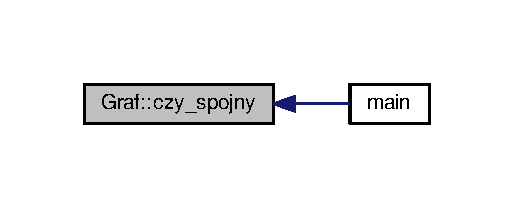
\includegraphics[width=246pt]{class_graf_ad83cd4b8656ccb75bd7b5f6cfe779080_icgraph}
\end{center}
\end{figure}


\hypertarget{class_graf_ad85c82918ac15887c9e423cd4edb1dba}{\index{Graf@{Graf}!dijkstry@{dijkstry}}
\index{dijkstry@{dijkstry}!Graf@{Graf}}
\subsubsection[{dijkstry}]{\setlength{\rightskip}{0pt plus 5cm}int Graf\-::dijkstry (
\begin{DoxyParamCaption}
\item[{int}]{a, }
\item[{int}]{b}
\end{DoxyParamCaption}
)}}\label{class_graf_ad85c82918ac15887c9e423cd4edb1dba}


Funkcja glowna programu wyszukujaca polaczenie. 

Funkcja wyszukuje polaczenie miedzy podanymi wierzcholkami 
\begin{DoxyParams}{Parameters}
{\em a} & -\/$>$ pole typu int z id wierzcholka z ktorego szukamy polaczenia \\
\hline
{\em b} & -\/$>$ pole typu int z id wierzcholka do ktorego szukamy polaczenia \\
\hline
\end{DoxyParams}
\begin{DoxyReturn}{Returns}
1 -\/$>$ gdy wystapi blad 0 -\/$>$ gdy bezblednie znajdzie polaczenie 
\end{DoxyReturn}


Definition at line 194 of file Dijkstry.\-cpp.



Here is the caller graph for this function\-:
\nopagebreak
\begin{figure}[H]
\begin{center}
\leavevmode
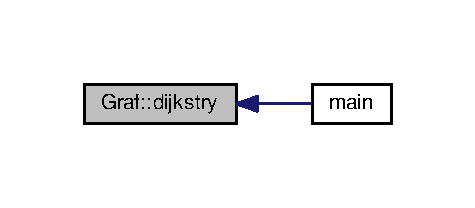
\includegraphics[width=228pt]{class_graf_ad85c82918ac15887c9e423cd4edb1dba_icgraph}
\end{center}
\end{figure}


\hypertarget{class_graf_a550437f8c2066ea035644502c93e1b7d}{\index{Graf@{Graf}!domyslny\-\_\-plik@{domyslny\-\_\-plik}}
\index{domyslny\-\_\-plik@{domyslny\-\_\-plik}!Graf@{Graf}}
\subsubsection[{domyslny\-\_\-plik}]{\setlength{\rightskip}{0pt plus 5cm}void Graf\-::domyslny\-\_\-plik (
\begin{DoxyParamCaption}
{}
\end{DoxyParamCaption}
)}}\label{class_graf_a550437f8c2066ea035644502c93e1b7d}


Funkcja pomocnicza do main . 

Funkcja jest tak naprawde tylko po to aby plik \hyperlink{main_8cpp}{main.\-cpp} byl bardziej przejrzysty Bierze domyslny plik (na chwile obecna jest to chyba plik fb.\-txt) i przerabia go, tworzy wierzcholki z niego i na koncu generuje polaczenia 

Definition at line 36 of file Dijkstry.\-cpp.



Here is the caller graph for this function\-:
\nopagebreak
\begin{figure}[H]
\begin{center}
\leavevmode
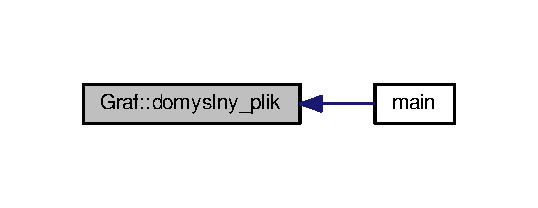
\includegraphics[width=258pt]{class_graf_a550437f8c2066ea035644502c93e1b7d_icgraph}
\end{center}
\end{figure}


\hypertarget{class_graf_ab1baac77bf17276ab97c721536dc4f33}{\index{Graf@{Graf}!dowolny\-\_\-plik@{dowolny\-\_\-plik}}
\index{dowolny\-\_\-plik@{dowolny\-\_\-plik}!Graf@{Graf}}
\subsubsection[{dowolny\-\_\-plik}]{\setlength{\rightskip}{0pt plus 5cm}void Graf\-::dowolny\-\_\-plik (
\begin{DoxyParamCaption}
{}
\end{DoxyParamCaption}
)}}\label{class_graf_ab1baac77bf17276ab97c721536dc4f33}


Funkcja pomocnicza do main . 

Funkcja jest tak naprawde tylko po to aby plik \hyperlink{main_8cpp}{main.\-cpp} byl bardziej przejrzysty Pyta o nazwe pliku, przerabia go, tworzy wierzcholki z niego i na koncu generuje polaczenia 

Definition at line 22 of file Dijkstry.\-cpp.



Here is the caller graph for this function\-:
\nopagebreak
\begin{figure}[H]
\begin{center}
\leavevmode
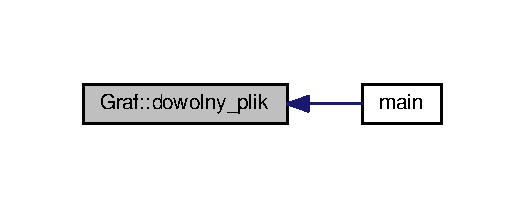
\includegraphics[width=252pt]{class_graf_ab1baac77bf17276ab97c721536dc4f33_icgraph}
\end{center}
\end{figure}


\hypertarget{class_graf_a2fe84bc61e57b1712687af6bda740103}{\index{Graf@{Graf}!generuj\-\_\-liste@{generuj\-\_\-liste}}
\index{generuj\-\_\-liste@{generuj\-\_\-liste}!Graf@{Graf}}
\subsubsection[{generuj\-\_\-liste}]{\setlength{\rightskip}{0pt plus 5cm}void Graf\-::generuj\-\_\-liste (
\begin{DoxyParamCaption}
\item[{int}]{ilosc, }
\item[{int}]{gestosc}
\end{DoxyParamCaption}
)}}\label{class_graf_a2fe84bc61e57b1712687af6bda740103}


Funkcja generujaca \hyperlink{class_graf}{Graf}. 

Funkcja typu void, na podstawie parametrow tworzy graf o zadanej losci \-: 
\begin{DoxyParams}{Parameters}
{\em ilosc} & -\/$>$ wartosc typu int przechowuje informacje o ilosci wierzchokow \\
\hline
{\em gestosc} & -\/$>$ wartosc typu int przechowuje informacje o gestosci polaczen w grafie \\
\hline
\end{DoxyParams}


Definition at line 337 of file Dijkstry.\-cpp.



Here is the caller graph for this function\-:
\nopagebreak
\begin{figure}[H]
\begin{center}
\leavevmode
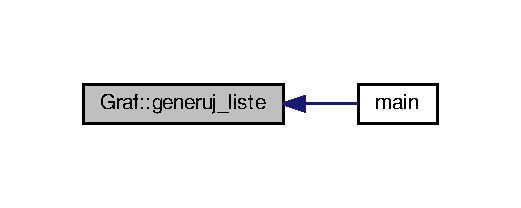
\includegraphics[width=250pt]{class_graf_a2fe84bc61e57b1712687af6bda740103_icgraph}
\end{center}
\end{figure}


\hypertarget{class_graf_aa66538b00c1915825b1e83339294c44e}{\index{Graf@{Graf}!losowe\-\_\-dijkstry@{losowe\-\_\-dijkstry}}
\index{losowe\-\_\-dijkstry@{losowe\-\_\-dijkstry}!Graf@{Graf}}
\subsubsection[{losowe\-\_\-dijkstry}]{\setlength{\rightskip}{0pt plus 5cm}void Graf\-::losowe\-\_\-dijkstry (
\begin{DoxyParamCaption}
{}
\end{DoxyParamCaption}
)}}\label{class_graf_aa66538b00c1915825b1e83339294c44e}


Funkcja pomocnicza do main . 

Funkcja jest tak naprawde tylko po to aby plik \hyperlink{main_8cpp}{main.\-cpp} byl bardziej przejrzysty Losuje wierzcholki miedzy ktorymi algorytm bedzie szukal polaczenie i nastepnie uruchamia go z tymi wartosciami 

Definition at line 59 of file Dijkstry.\-cpp.



Here is the caller graph for this function\-:
\nopagebreak
\begin{figure}[H]
\begin{center}
\leavevmode
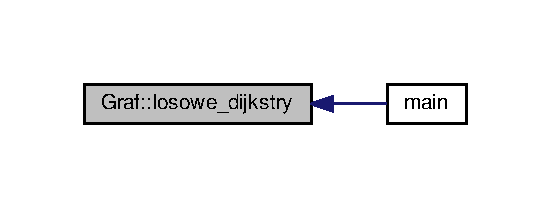
\includegraphics[width=264pt]{class_graf_aa66538b00c1915825b1e83339294c44e_icgraph}
\end{center}
\end{figure}


\hypertarget{class_graf_a7997ef54e93c3b83a2435bfd0d4c51c8}{\index{Graf@{Graf}!przerob\-\_\-z\-\_\-fb@{przerob\-\_\-z\-\_\-fb}}
\index{przerob\-\_\-z\-\_\-fb@{przerob\-\_\-z\-\_\-fb}!Graf@{Graf}}
\subsubsection[{przerob\-\_\-z\-\_\-fb}]{\setlength{\rightskip}{0pt plus 5cm}void Graf\-::przerob\-\_\-z\-\_\-fb (
\begin{DoxyParamCaption}
\item[{string}]{typ, }
\item[{string}]{wyjscie}
\end{DoxyParamCaption}
)}}\label{class_graf_a7997ef54e93c3b83a2435bfd0d4c51c8}


Funkcja przerabiajaca plik z bazy . 

Funkcja typu void, tworzaca wierzcholki z pliku, gdzie sa podane tylko wierzcholki 
\begin{DoxyParams}{Parameters}
{\em typ} & -\/$>$ wartosc typu string przechowuje nazwe pliku wejsciowego, ktorego bedziemy obrabiac \\
\hline
{\em wyjscie} & -\/$>$ wartosc typu string przechowuje nazwe pliku przerobionego ( nowo stworzonego ) \\
\hline
\end{DoxyParams}


Definition at line 69 of file Dijkstry.\-cpp.

\hypertarget{class_graf_ae3cb2f3d4a8c9cc67845eacacf6a612d}{\index{Graf@{Graf}!przypisz\-\_\-indeks@{przypisz\-\_\-indeks}}
\index{przypisz\-\_\-indeks@{przypisz\-\_\-indeks}!Graf@{Graf}}
\subsubsection[{przypisz\-\_\-indeks}]{\setlength{\rightskip}{0pt plus 5cm}int Graf\-::przypisz\-\_\-indeks (
\begin{DoxyParamCaption}
\item[{int}]{id}
\end{DoxyParamCaption}
)}}\label{class_graf_ae3cb2f3d4a8c9cc67845eacacf6a612d}


Funkcja pomocnicza. 

Funkcja sluzy do przypisania indeksu wierzcholkowi po podanym id 
\begin{DoxyParams}{Parameters}
{\em id} & -\/$>$ pole typu int z id wierzcholka \\
\hline
\end{DoxyParams}
\begin{DoxyReturn}{Returns}
indeks -\/$>$ mniejszy musi byc niz ilosc wierzcholkow 
\end{DoxyReturn}


Definition at line 138 of file Dijkstry.\-cpp.

\hypertarget{class_graf_adaba0ec276dc425b2556f2dadae7845f}{\index{Graf@{Graf}!stworz\-\_\-liste\-\_\-z\-\_\-pliku@{stworz\-\_\-liste\-\_\-z\-\_\-pliku}}
\index{stworz\-\_\-liste\-\_\-z\-\_\-pliku@{stworz\-\_\-liste\-\_\-z\-\_\-pliku}!Graf@{Graf}}
\subsubsection[{stworz\-\_\-liste\-\_\-z\-\_\-pliku}]{\setlength{\rightskip}{0pt plus 5cm}void Graf\-::stworz\-\_\-liste\-\_\-z\-\_\-pliku (
\begin{DoxyParamCaption}
\item[{string}]{nazwapliku}
\end{DoxyParamCaption}
)}}\label{class_graf_adaba0ec276dc425b2556f2dadae7845f}


Funkcja tworzaca \hyperlink{class_graf}{Graf} z pliku. 

Funkcja typu void, tworzaca graf z pliku, gdzie sa podane polaczenia miedzy wierzcholkami ( tylko ) 
\begin{DoxyParams}{Parameters}
{\em nazwapliku} & -\/$>$ wartosc typu string przechowuje nazwe pliku \\
\hline
\end{DoxyParams}


Definition at line 95 of file Dijkstry.\-cpp.

\hypertarget{class_graf_a3fee2a8a88543338f1d54216c2618e2b}{\index{Graf@{Graf}!stworz\-\_\-wierzcholki@{stworz\-\_\-wierzcholki}}
\index{stworz\-\_\-wierzcholki@{stworz\-\_\-wierzcholki}!Graf@{Graf}}
\subsubsection[{stworz\-\_\-wierzcholki}]{\setlength{\rightskip}{0pt plus 5cm}void Graf\-::stworz\-\_\-wierzcholki (
\begin{DoxyParamCaption}
\item[{string}]{nazwapliku}
\end{DoxyParamCaption}
)}}\label{class_graf_a3fee2a8a88543338f1d54216c2618e2b}


Funkcja tworzaca wierzcholki \hyperlink{class_graf}{Graf} u z pliku. 

Funkcja typu void, tworzaca wierzcholki z pliku, gdzie sa podane tylko wierzcholki 
\begin{DoxyParams}{Parameters}
{\em nazwapliku} & -\/$>$ wartosc typu string przechowuje nazwe pliku \\
\hline
\end{DoxyParams}


Definition at line 150 of file Dijkstry.\-cpp.

\hypertarget{class_graf_a8a0677ac53fdef2117a52da0f944701a}{\index{Graf@{Graf}!testowy\-\_\-plik@{testowy\-\_\-plik}}
\index{testowy\-\_\-plik@{testowy\-\_\-plik}!Graf@{Graf}}
\subsubsection[{testowy\-\_\-plik}]{\setlength{\rightskip}{0pt plus 5cm}void Graf\-::testowy\-\_\-plik (
\begin{DoxyParamCaption}
{}
\end{DoxyParamCaption}
)}}\label{class_graf_a8a0677ac53fdef2117a52da0f944701a}


Funkcja pomocnicza do main . 

Funkcja jest tak naprawde tylko po to aby plik \hyperlink{main_8cpp}{main.\-cpp} byl bardziej przejrzysty Bierze plik testowy ( test.\-txt ) przerabia go, tworzy wierzcholki z niego i na koncu generuje polaczenia 

Definition at line 47 of file Dijkstry.\-cpp.



Here is the caller graph for this function\-:
\nopagebreak
\begin{figure}[H]
\begin{center}
\leavevmode
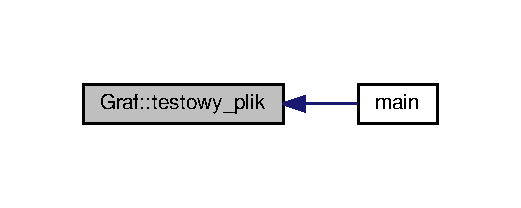
\includegraphics[width=250pt]{class_graf_a8a0677ac53fdef2117a52da0f944701a_icgraph}
\end{center}
\end{figure}


\hypertarget{class_graf_a3a084b33cfcfa17bbfc05570043aaab2}{\index{Graf@{Graf}!wyswietl@{wyswietl}}
\index{wyswietl@{wyswietl}!Graf@{Graf}}
\subsubsection[{wyswietl}]{\setlength{\rightskip}{0pt plus 5cm}void Graf\-::wyswietl (
\begin{DoxyParamCaption}
{}
\end{DoxyParamCaption}
)}}\label{class_graf_a3a084b33cfcfa17bbfc05570043aaab2}


Funkcja wyswietlajaca liste sasiedztwa grafu. 

Funkcja typu void wyswietla aktualny stan grafu. 

Definition at line 163 of file Dijkstry.\-cpp.



Here is the caller graph for this function\-:
\nopagebreak
\begin{figure}[H]
\begin{center}
\leavevmode
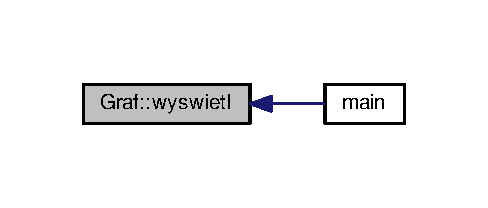
\includegraphics[width=234pt]{class_graf_a3a084b33cfcfa17bbfc05570043aaab2_icgraph}
\end{center}
\end{figure}




\subsection{Member Data Documentation}
\hypertarget{class_graf_a30dc3bf4726fbd2d056c98f15080b236}{\index{Graf@{Graf}!E@{E}}
\index{E@{E}!Graf@{Graf}}
\subsubsection[{E}]{\setlength{\rightskip}{0pt plus 5cm}int Graf\-::\-E}}\label{class_graf_a30dc3bf4726fbd2d056c98f15080b236}


Pole typu int, bedzie uzywane do przechowywania informacji o ilosci krawedzi (aktualnie nie uzywane w programie ). 



Definition at line 85 of file Dijkstry.\-hh.

\hypertarget{class_graf_adf576dd4fd3cb35f4328a66befaa9c7a}{\index{Graf@{Graf}!lista\-\_\-sasiadujaca@{lista\-\_\-sasiadujaca}}
\index{lista\-\_\-sasiadujaca@{lista\-\_\-sasiadujaca}!Graf@{Graf}}
\subsubsection[{lista\-\_\-sasiadujaca}]{\setlength{\rightskip}{0pt plus 5cm}vector$<${\bf Wierzcholek}$>$$\ast$ Graf\-::lista\-\_\-sasiadujaca}}\label{class_graf_adf576dd4fd3cb35f4328a66befaa9c7a}


Pole typu $\ast$ vector, bedzie uzywane do przechowywania informacji o sasiadach dla poszczegolnych wierzcholkow. 



Definition at line 89 of file Dijkstry.\-hh.

\hypertarget{class_graf_a673185b62d4c232bcbbc0200e95e7481}{\index{Graf@{Graf}!V@{V}}
\index{V@{V}!Graf@{Graf}}
\subsubsection[{V}]{\setlength{\rightskip}{0pt plus 5cm}int Graf\-::\-V}}\label{class_graf_a673185b62d4c232bcbbc0200e95e7481}


Pole typu int, bedzie uzywane do przechowywania informacji o ilosci wierzcholkow. 



Definition at line 81 of file Dijkstry.\-hh.

\hypertarget{class_graf_a2df9c551c0ed169e20bdfe06aba56558}{\index{Graf@{Graf}!wierzcholki@{wierzcholki}}
\index{wierzcholki@{wierzcholki}!Graf@{Graf}}
\subsubsection[{wierzcholki}]{\setlength{\rightskip}{0pt plus 5cm}int$\ast$ Graf\-::wierzcholki}}\label{class_graf_a2df9c551c0ed169e20bdfe06aba56558}


Pole typu $\ast$ int, bedzie uzywane jako wektor z prawdziwymi nazwami (id) wierzcholkow. 



Definition at line 93 of file Dijkstry.\-hh.



The documentation for this class was generated from the following files\-:\begin{DoxyCompactItemize}
\item 
/home/pawel/\-Dokumenty/programowanie/pamsi/projekt\-\_\-znajomi/prj/inc/\hyperlink{_dijkstry_8hh}{Dijkstry.\-hh}\item 
/home/pawel/\-Dokumenty/programowanie/pamsi/projekt\-\_\-znajomi/prj/src/\hyperlink{_dijkstry_8cpp}{Dijkstry.\-cpp}\end{DoxyCompactItemize}

\hypertarget{structpor}{\section{por Struct Reference}
\label{structpor}\index{por@{por}}
}


Struktura porownywania Struktura ta ma na celu ulatwienie dzialania algorytmu wyszukiwania ( Dijkstry ) Prownuje ona wartosci drogi miedzy dwoma wezlami.  




{\ttfamily \#include $<$Dijkstry.\-hh$>$}

\subsection*{Public Member Functions}
\begin{DoxyCompactItemize}
\item 
bool \hyperlink{structpor_a35a4b60c898e387cd101e40dda33c599}{operator()} (const \hyperlink{struct_wezel}{Wezel} \&k1, const \hyperlink{struct_wezel}{Wezel} \&k2)
\end{DoxyCompactItemize}


\subsection{Detailed Description}
Struktura porownywania Struktura ta ma na celu ulatwienie dzialania algorytmu wyszukiwania ( Dijkstry ) Prownuje ona wartosci drogi miedzy dwoma wezlami. 

Definition at line 244 of file Dijkstry.\-hh.



\subsection{Member Function Documentation}
\hypertarget{structpor_a35a4b60c898e387cd101e40dda33c599}{\index{por@{por}!operator()@{operator()}}
\index{operator()@{operator()}!por@{por}}
\subsubsection[{operator()}]{\setlength{\rightskip}{0pt plus 5cm}bool por\-::operator() (
\begin{DoxyParamCaption}
\item[{const {\bf Wezel} \&}]{k1, }
\item[{const {\bf Wezel} \&}]{k2}
\end{DoxyParamCaption}
)\hspace{0.3cm}{\ttfamily [inline]}}}\label{structpor_a35a4b60c898e387cd101e40dda33c599}


Definition at line 245 of file Dijkstry.\-hh.



The documentation for this struct was generated from the following file\-:\begin{DoxyCompactItemize}
\item 
/home/pawel/\-Dokumenty/programowanie/pamsi/projekt\-\_\-znajomi/prj/inc/\hyperlink{_dijkstry_8hh}{Dijkstry.\-hh}\end{DoxyCompactItemize}

\hypertarget{struct_wezel}{\section{Wezel Struct Reference}
\label{struct_wezel}\index{Wezel@{Wezel}}
}


Struktura Wezla Struktura ta ma zdefiniowane dwie zmienne nr oraz g, ktore odpowiadaja za przechowywanie numer wierzcholkana oraz droge jaka juz przebyl od poczatku dzialania wyszukiwania.  




{\ttfamily \#include $<$Dijkstry.\-hh$>$}

\subsection*{Public Attributes}
\begin{DoxyCompactItemize}
\item 
int \hyperlink{struct_wezel_ab6bc8ea479ff25001606d388bbd7ccd0}{nr}
\begin{DoxyCompactList}\small\item\em Pole typu int, bedzie uzywane do przechowywania id wierzcholka. \end{DoxyCompactList}\item 
int \hyperlink{struct_wezel_ab8cc87757f857deaca9fdb3842b0c455}{g}
\begin{DoxyCompactList}\small\item\em Pole typu int, bedzie uzywane do przechowywania informacji o przebytej drodze. \end{DoxyCompactList}\end{DoxyCompactItemize}


\subsection{Detailed Description}
Struktura Wezla Struktura ta ma zdefiniowane dwie zmienne nr oraz g, ktore odpowiadaja za przechowywanie numer wierzcholkana oraz droge jaka juz przebyl od poczatku dzialania wyszukiwania. 

Definition at line 60 of file Dijkstry.\-hh.



\subsection{Member Data Documentation}
\hypertarget{struct_wezel_ab8cc87757f857deaca9fdb3842b0c455}{\index{Wezel@{Wezel}!g@{g}}
\index{g@{g}!Wezel@{Wezel}}
\subsubsection[{g}]{\setlength{\rightskip}{0pt plus 5cm}int Wezel\-::g}}\label{struct_wezel_ab8cc87757f857deaca9fdb3842b0c455}


Pole typu int, bedzie uzywane do przechowywania informacji o przebytej drodze. 



Definition at line 68 of file Dijkstry.\-hh.

\hypertarget{struct_wezel_ab6bc8ea479ff25001606d388bbd7ccd0}{\index{Wezel@{Wezel}!nr@{nr}}
\index{nr@{nr}!Wezel@{Wezel}}
\subsubsection[{nr}]{\setlength{\rightskip}{0pt plus 5cm}int Wezel\-::nr}}\label{struct_wezel_ab6bc8ea479ff25001606d388bbd7ccd0}


Pole typu int, bedzie uzywane do przechowywania id wierzcholka. 



Definition at line 64 of file Dijkstry.\-hh.



The documentation for this struct was generated from the following file\-:\begin{DoxyCompactItemize}
\item 
/home/pawel/\-Dokumenty/programowanie/pamsi/projekt\-\_\-znajomi/prj/inc/\hyperlink{_dijkstry_8hh}{Dijkstry.\-hh}\end{DoxyCompactItemize}

\hypertarget{class_wierzcholek}{\section{Wierzcholek Class Reference}
\label{class_wierzcholek}\index{Wierzcholek@{Wierzcholek}}
}


Definicje dla klasy \hyperlink{class_wierzcholek}{Wierzcholek} Struktura ta ma zdefiniowane dwie zmienne sasiad oraz waga. Przy wczytywaniu pliku dodajac wierzcholek dodajemy odrazu informacje o aktualnym sasiedzie oraz o wadze polaczenia miedzy wierzcholkiem i sasiadem.  




{\ttfamily \#include $<$Dijkstry.\-hh$>$}

\subsection*{Public Member Functions}
\begin{DoxyCompactItemize}
\item 
\hyperlink{class_wierzcholek_aecbad5c4116749559a7b57888fab2f01}{Wierzcholek} ()
\begin{DoxyCompactList}\small\item\em Konstruktor klasy \hyperlink{class_wierzcholek}{Wierzcholek}. \end{DoxyCompactList}\item 
\hyperlink{class_wierzcholek}{Wierzcholek} \& \hyperlink{class_wierzcholek_a8ed21ba858df5ba6857b22f9a95929d8}{operator=} (\hyperlink{class_wierzcholek}{Wierzcholek} const \&c1)
\begin{DoxyCompactList}\small\item\em Funkcja przeciazajaca operator '='. \end{DoxyCompactList}\end{DoxyCompactItemize}
\subsection*{Public Attributes}
\begin{DoxyCompactItemize}
\item 
int \hyperlink{class_wierzcholek_a064e9d988e2bf41110c06f50ee4a7549}{sasiad}
\begin{DoxyCompactList}\small\item\em Pole typu int, bedzie uzywane do numeru id sasiada dla danego wierzcholka. \end{DoxyCompactList}\item 
int \hyperlink{class_wierzcholek_a75fca22ce5c86f0cbf29276f7f5204c3}{waga}
\begin{DoxyCompactList}\small\item\em Pole typu int, bedzie uzywane do przechowywania informacji o wadze polaczenia. \end{DoxyCompactList}\end{DoxyCompactItemize}


\subsection{Detailed Description}
Definicje dla klasy \hyperlink{class_wierzcholek}{Wierzcholek} Struktura ta ma zdefiniowane dwie zmienne sasiad oraz waga. Przy wczytywaniu pliku dodajac wierzcholek dodajemy odrazu informacje o aktualnym sasiedzie oraz o wadze polaczenia miedzy wierzcholkiem i sasiadem. 

Definition at line 29 of file Dijkstry.\-hh.



\subsection{Constructor \& Destructor Documentation}
\hypertarget{class_wierzcholek_aecbad5c4116749559a7b57888fab2f01}{\index{Wierzcholek@{Wierzcholek}!Wierzcholek@{Wierzcholek}}
\index{Wierzcholek@{Wierzcholek}!Wierzcholek@{Wierzcholek}}
\subsubsection[{Wierzcholek}]{\setlength{\rightskip}{0pt plus 5cm}Wierzcholek\-::\-Wierzcholek (
\begin{DoxyParamCaption}
{}
\end{DoxyParamCaption}
)\hspace{0.3cm}{\ttfamily [inline]}}}\label{class_wierzcholek_aecbad5c4116749559a7b57888fab2f01}


Konstruktor klasy \hyperlink{class_wierzcholek}{Wierzcholek}. 

Konstruktor jest bezparametryczny. Wykonuje wyzerowanie wszystkich skladowych wewnwetrznych klasy 

Definition at line 46 of file Dijkstry.\-hh.



\subsection{Member Function Documentation}
\hypertarget{class_wierzcholek_a8ed21ba858df5ba6857b22f9a95929d8}{\index{Wierzcholek@{Wierzcholek}!operator=@{operator=}}
\index{operator=@{operator=}!Wierzcholek@{Wierzcholek}}
\subsubsection[{operator=}]{\setlength{\rightskip}{0pt plus 5cm}{\bf Wierzcholek} \& Wierzcholek\-::operator= (
\begin{DoxyParamCaption}
\item[{{\bf Wierzcholek} const \&}]{c1}
\end{DoxyParamCaption}
)}}\label{class_wierzcholek_a8ed21ba858df5ba6857b22f9a95929d8}


Funkcja przeciazajaca operator '='. 



Definition at line 281 of file Dijkstry.\-cpp.



\subsection{Member Data Documentation}
\hypertarget{class_wierzcholek_a064e9d988e2bf41110c06f50ee4a7549}{\index{Wierzcholek@{Wierzcholek}!sasiad@{sasiad}}
\index{sasiad@{sasiad}!Wierzcholek@{Wierzcholek}}
\subsubsection[{sasiad}]{\setlength{\rightskip}{0pt plus 5cm}int Wierzcholek\-::sasiad}}\label{class_wierzcholek_a064e9d988e2bf41110c06f50ee4a7549}


Pole typu int, bedzie uzywane do numeru id sasiada dla danego wierzcholka. 



Definition at line 34 of file Dijkstry.\-hh.

\hypertarget{class_wierzcholek_a75fca22ce5c86f0cbf29276f7f5204c3}{\index{Wierzcholek@{Wierzcholek}!waga@{waga}}
\index{waga@{waga}!Wierzcholek@{Wierzcholek}}
\subsubsection[{waga}]{\setlength{\rightskip}{0pt plus 5cm}int Wierzcholek\-::waga}}\label{class_wierzcholek_a75fca22ce5c86f0cbf29276f7f5204c3}


Pole typu int, bedzie uzywane do przechowywania informacji o wadze polaczenia. 



Definition at line 38 of file Dijkstry.\-hh.



The documentation for this class was generated from the following files\-:\begin{DoxyCompactItemize}
\item 
/home/pawel/\-Dokumenty/programowanie/pamsi/projekt\-\_\-znajomi/prj/inc/\hyperlink{_dijkstry_8hh}{Dijkstry.\-hh}\item 
/home/pawel/\-Dokumenty/programowanie/pamsi/projekt\-\_\-znajomi/prj/src/\hyperlink{_dijkstry_8cpp}{Dijkstry.\-cpp}\end{DoxyCompactItemize}

\chapter{File Documentation}
\hypertarget{strona_8dox}{\section{/home/pawel/\-Dokumenty/programowanie/pamsi/sortowanie/prj/doc/pages/strona.dox File Reference}
\label{strona_8dox}\index{/home/pawel/\-Dokumenty/programowanie/pamsi/sortowanie/prj/doc/pages/strona.\-dox@{/home/pawel/\-Dokumenty/programowanie/pamsi/sortowanie/prj/doc/pages/strona.\-dox}}
}

\hypertarget{_dijkstry_8hh}{\section{/home/pawel/\-Dokumenty/programowanie/pamsi/projekt\-\_\-znajomi/prj/inc/\-Dijkstry.hh File Reference}
\label{_dijkstry_8hh}\index{/home/pawel/\-Dokumenty/programowanie/pamsi/projekt\-\_\-znajomi/prj/inc/\-Dijkstry.\-hh@{/home/pawel/\-Dokumenty/programowanie/pamsi/projekt\-\_\-znajomi/prj/inc/\-Dijkstry.\-hh}}
}


Definicje funkcji dla klasy graf.  


{\ttfamily \#include $<$iostream$>$}\\*
{\ttfamily \#include $<$fstream$>$}\\*
{\ttfamily \#include $<$vector$>$}\\*
{\ttfamily \#include $<$algorithm$>$}\\*
{\ttfamily \#include $<$iomanip$>$}\\*
{\ttfamily \#include $<$stack$>$}\\*
{\ttfamily \#include $<$queue$>$}\\*
{\ttfamily \#include $<$ctime$>$}\\*
Include dependency graph for Dijkstry.\-hh\-:
\nopagebreak
\begin{figure}[H]
\begin{center}
\leavevmode
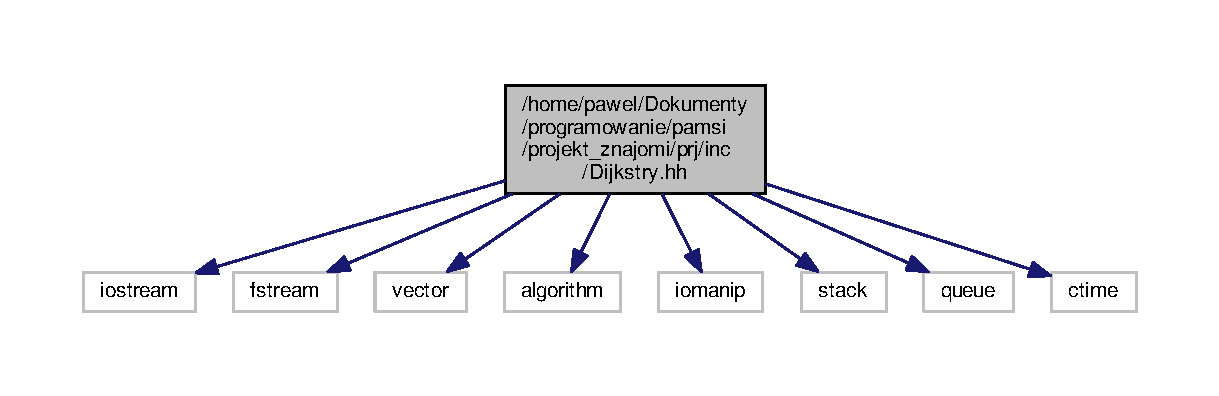
\includegraphics[width=350pt]{_dijkstry_8hh__incl}
\end{center}
\end{figure}
This graph shows which files directly or indirectly include this file\-:
\nopagebreak
\begin{figure}[H]
\begin{center}
\leavevmode
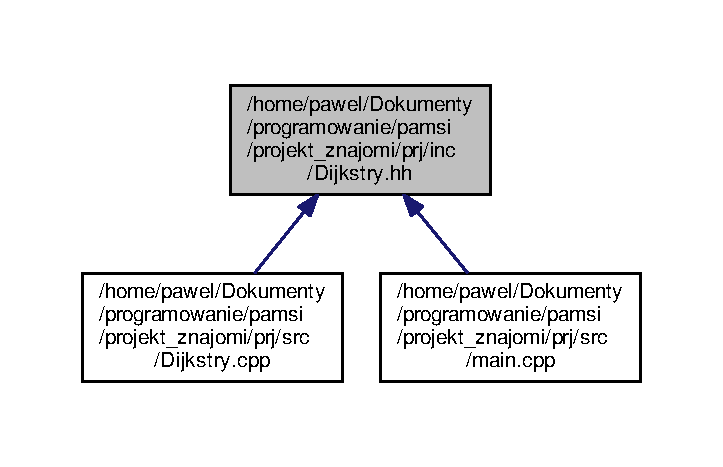
\includegraphics[width=347pt]{_dijkstry_8hh__dep__incl}
\end{center}
\end{figure}
\subsection*{Classes}
\begin{DoxyCompactItemize}
\item 
class \hyperlink{class_wierzcholek}{Wierzcholek}
\begin{DoxyCompactList}\small\item\em Definicje dla klasy \hyperlink{class_wierzcholek}{Wierzcholek} Struktura ta ma zdefiniowane dwie zmienne sasiad oraz waga. Przy wczytywaniu pliku dodajac wierzcholek dodajemy odrazu informacje o aktualnym sasiedzie oraz o wadze polaczenia miedzy wierzcholkiem i sasiadem. \end{DoxyCompactList}\item 
struct \hyperlink{struct_wezel}{Wezel}
\begin{DoxyCompactList}\small\item\em Struktura Wezla Struktura ta ma zdefiniowane dwie zmienne nr oraz g, ktore odpowiadaja za przechowywanie numer wierzcholkana oraz droge jaka juz przebyl od poczatku dzialania wyszukiwania. \end{DoxyCompactList}\item 
class \hyperlink{class_graf}{Graf}
\begin{DoxyCompactList}\small\item\em Modeluje pojecie graf. Klasa sluzy glownie do wykonania algorytmu wyszukiwania, czyli znalezienia polaczenia miedzy dwoma punktami. \end{DoxyCompactList}\item 
struct \hyperlink{structpor}{por}
\begin{DoxyCompactList}\small\item\em Struktura porownywania Struktura ta ma na celu ulatwienie dzialania algorytmu wyszukiwania ( Dijkstry ) Prownuje ona wartosci drogi miedzy dwoma wezlami. \end{DoxyCompactList}\end{DoxyCompactItemize}


\subsection{Detailed Description}
Definicje funkcji dla klasy graf. 

Definition in file \hyperlink{_dijkstry_8hh_source}{Dijkstry.\-hh}.


\hypertarget{_dijkstry_8cpp}{\section{/home/pawel/\-Dokumenty/programowanie/pamsi/projekt\-\_\-znajomi/prj/src/\-Dijkstry.cpp File Reference}
\label{_dijkstry_8cpp}\index{/home/pawel/\-Dokumenty/programowanie/pamsi/projekt\-\_\-znajomi/prj/src/\-Dijkstry.\-cpp@{/home/pawel/\-Dokumenty/programowanie/pamsi/projekt\-\_\-znajomi/prj/src/\-Dijkstry.\-cpp}}
}


Plik zawiera funkcje z klasy graf.  


{\ttfamily \#include \char`\"{}../inc/\-Dijkstry.\-hh\char`\"{}}\\*
Include dependency graph for Dijkstry.\-cpp\-:
\nopagebreak
\begin{figure}[H]
\begin{center}
\leavevmode
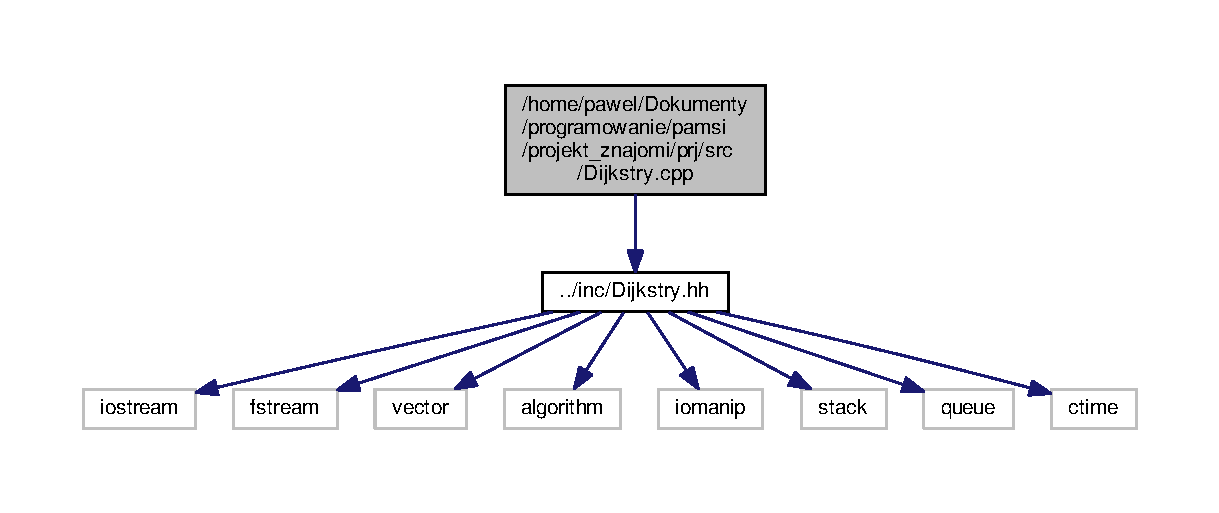
\includegraphics[width=350pt]{_dijkstry_8cpp__incl}
\end{center}
\end{figure}


\subsection{Detailed Description}
Plik zawiera funkcje z klasy graf. 

Definition in file \hyperlink{_dijkstry_8cpp_source}{Dijkstry.\-cpp}.


\hypertarget{main_8cpp}{\section{/home/pawel/\-Dokumenty/programowanie/pamsi/simplex/prj/src/main.cpp File Reference}
\label{main_8cpp}\index{/home/pawel/\-Dokumenty/programowanie/pamsi/simplex/prj/src/main.\-cpp@{/home/pawel/\-Dokumenty/programowanie/pamsi/simplex/prj/src/main.\-cpp}}
}


Plik zawiera funkcje \hyperlink{main_8cpp_ae66f6b31b5ad750f1fe042a706a4e3d4}{main()}  


{\ttfamily \#include $<$iostream$>$}\\*
{\ttfamily \#include \char`\"{}../inc/simplex.\-hh\char`\"{}}\\*
Include dependency graph for main.\-cpp\-:\nopagebreak
\begin{figure}[H]
\begin{center}
\leavevmode
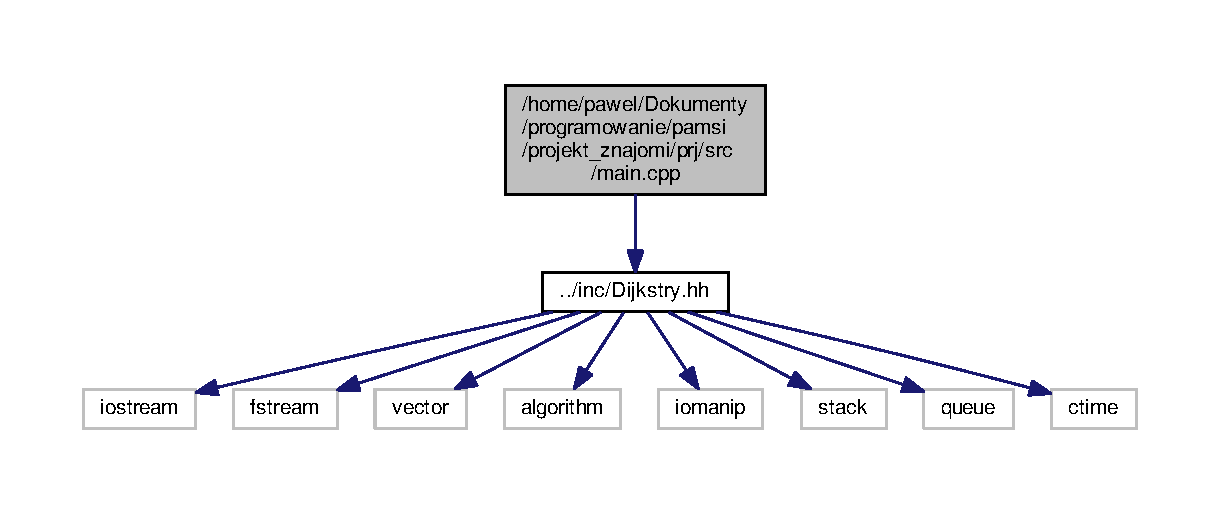
\includegraphics[width=224pt]{main_8cpp__incl}
\end{center}
\end{figure}
\subsection*{Functions}
\begin{DoxyCompactItemize}
\item 
int \hyperlink{main_8cpp_ae66f6b31b5ad750f1fe042a706a4e3d4}{main} ()
\end{DoxyCompactItemize}


\subsection{Detailed Description}
Plik zawiera funkcje \hyperlink{main_8cpp_ae66f6b31b5ad750f1fe042a706a4e3d4}{main()} 

Definition in file \hyperlink{main_8cpp_source}{main.\-cpp}.



\subsection{Function Documentation}
\hypertarget{main_8cpp_ae66f6b31b5ad750f1fe042a706a4e3d4}{\index{main.\-cpp@{main.\-cpp}!main@{main}}
\index{main@{main}!main.cpp@{main.\-cpp}}
\subsubsection[{main}]{\setlength{\rightskip}{0pt plus 5cm}int main (
\begin{DoxyParamCaption}
{}
\end{DoxyParamCaption}
)}}\label{main_8cpp_ae66f6b31b5ad750f1fe042a706a4e3d4}


Definition at line 13 of file main.\-cpp.



Here is the call graph for this function\-:\nopagebreak
\begin{figure}[H]
\begin{center}
\leavevmode
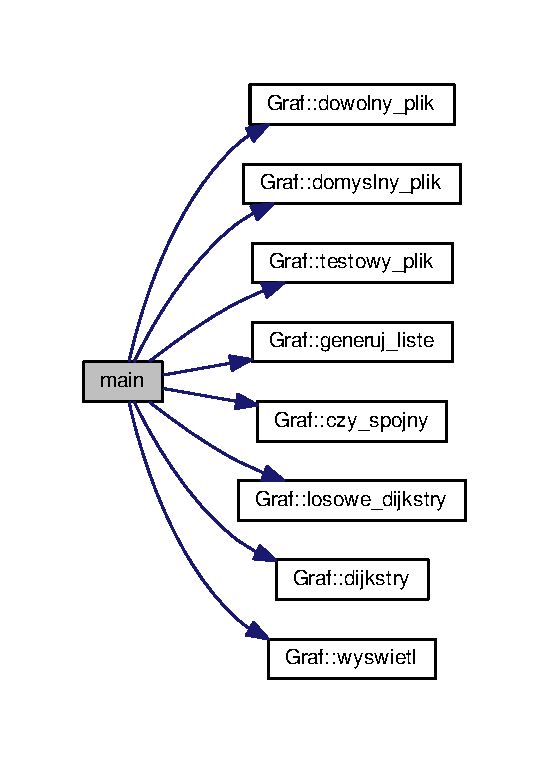
\includegraphics[width=282pt]{main_8cpp_ae66f6b31b5ad750f1fe042a706a4e3d4_cgraph}
\end{center}
\end{figure}



%--- End generated contents ---

% Index
\newpage
\phantomsection
\addcontentsline{toc}{chapter}{Index}
\printindex

\end{document}
